% generated by scripts/pkl_to_latex.py
% source PKL : uscan_v1_L6_Ne6_t0p1_mode-uniform_nmin2_solver-gcg_full_restarts8_iter300_kmax2_tol1em09_U0to15_N16-2f7c06936fa2.pkl
% scan type  : uscan
% state      : gs
% requires   : \usepackage{pgfplots} \pgfplotsset{compat=1.18}
% colours match the matplotlib PDF (tab10 cycle)
\definecolor{gmeC0}{HTML}{1F77B4}
\definecolor{gmeC1}{HTML}{FF7F0E}
\definecolor{gmeC2}{HTML}{2CA02C}
\definecolor{gmeC3}{HTML}{D62728}
\definecolor{gmeC4}{HTML}{9467BD}
\definecolor{gmeC5}{HTML}{8C564B}
\definecolor{gmeC6}{HTML}{E377C2}
\definecolor{gmeC7}{HTML}{17BECF}

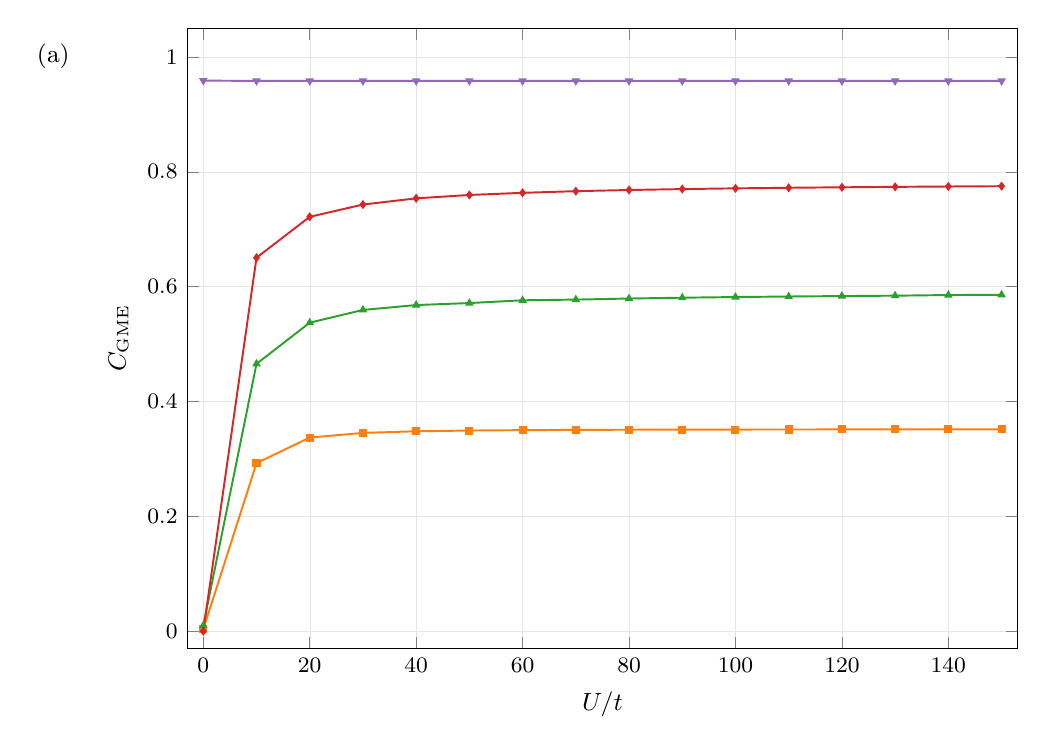
\begin{tikzpicture}
  \begin{axis}[
    width=\columnwidth,
    height=0.78\columnwidth,
    xlabel={$U/t$},
    ylabel={$C_{\mathrm{GME}}$},
    grid=both,
    grid style={line width=.1pt, draw=gray!20},
    tick label style={font=\footnotesize\rmfamily, /pgf/number format/fixed},
    label style={font=\small\rmfamily},
    scaled ticks=false,
    legend style={font=\scriptsize\rmfamily, draw=gray!40, at={(0.5,1.03)}, anchor=south, /tikz/every even column/.append style={column sep=6pt}},
    legend cell align={left},
    legend columns=2,
    ymin=-0.03,
    ymax=1.05,
    xmin=-3,
    xmax=153,
    after end axis/.append code={\node[anchor=east, font=\small\rmfamily] at (axis description cs:-0.13,0.954) {(a)};},
  ]
    \addplot[color=gmeC1, mark=square*, mark size=1.1pt, line width=0.7pt] coordinates {
        (0,0.003277) (10,0.292503) (20,0.337214) (30,0.345268)
        (40,0.348079) (50,0.349379) (60,0.350086) (70,0.350511)
        (80,0.350788) (90,0.350977) (100,0.351113) (110,0.351213)
        (120,0.351289) (130,0.351349) (140,0.351396) (150,0.351434)
    };
    \addplot[color=gmeC2, mark=triangle*, mark size=1.1pt, line width=0.7pt] coordinates {
        (0,0.009808) (10,0.465513) (20,0.53721) (30,0.559378)
        (40,0.567936) (50,0.571384) (60,0.576212) (70,0.577415)
        (80,0.579277) (90,0.580718) (100,0.581865) (110,0.582802)
        (120,0.583578) (130,0.584236) (140,0.58536) (150,0.58581)
    };
    \addplot[color=gmeC3, mark=diamond*, mark size=1.1pt, line width=0.7pt] coordinates {
        (0,0) (10,0.650349) (20,0.721531) (30,0.742946)
        (40,0.753744) (50,0.759606) (60,0.76336) (70,0.766221)
        (80,0.768269) (90,0.769856) (100,0.771122) (110,0.772154)
        (120,0.772983) (130,0.773735) (140,0.77436) (150,0.774897)
    };
    \addplot[color=gmeC4, mark=triangle*, mark size=1.1pt, mark options={rotate=180}, line width=0.7pt] coordinates {
        (0,0.95878) (10,0.958182) (20,0.958179) (30,0.958179)
        (40,0.958179) (50,0.958179) (60,0.958179) (70,0.958179)
        (80,0.958179) (90,0.958179) (100,0.958179) (110,0.958179)
        (120,0.958179) (130,0.958179) (140,0.958179) (150,0.958179)
    };
  \end{axis}
\end{tikzpicture}
